\documentclass[10pt]{article}
\usepackage[utf8]{inputenc}
\usepackage[T1]{fontenc}
\usepackage{amsmath}
\usepackage{amsfonts}
\usepackage{amssymb}
\usepackage[version=4]{mhchem}
\usepackage{stmaryrd}
\usepackage{graphicx}
\usepackage[export]{adjustbox}
\graphicspath{ {./images/} }

\title{$07 / 25 / 19$ }

\author{}
\date{}


\begin{document}
\maketitle
Sample Test Questions

The following questions are provided as examples of the types of questions that might be covered on your certification exam. These questions may help prepare you for certification by identifying areas in which you need additional study. The correct answers and reference material for each question are found in the following section. If you cannot answer a question correctly, read the reference material listed for the question. The reference material will help you better understand the topic and may help you answer similar questions that may be on the certification exam.

It is unlikely that you will find any of these question duplicated on a certification exam, so don't try to memorize the questions and answers. Many operators find it is helpful to contact their State Certification Program listed in the last section of the guidebook to request information about the certification exam. Some, but not all, certification programs will provide a list of suggested study material, topics covered on the exam and sample exam questions.

These sample questions should not be used in place of other training materials and courses. The "Training Opportunities and Resources" section of this guidebook contains additional information.

\begin{enumerate}
  \item If a customer complains about the drinking water characteristics, the operator should record the complaint and
\end{enumerate}

(A.) Investigate inmediately

B. Investigate only if more complaints are received

C. Inform the customer that the water should be boiled

D. Inform the customer that the water is safe

\begin{enumerate}
  \setcounter{enumi}{1}
  \item What term is used when a water utility divides its total operating expenses into the total revenue?\\
A. Debt ratio\\
(B.) Operating ratio\\
C. Credit ratio\\
,D. Coverage ratio

  \item How often should operation data, such as flow rate, amount of water treated; dosage of chemical, and reservoir levels be recorded?\\
A. Twice a day\\
(B.) Daily\\
C. Weekly\\
D. Monthly

  \item Which of the following is the most important reason to keep daily records of operational data?\\
A. Maintain records for customer billing\\
B. Document the need for an increased budget\\
C. Provide insurance data\\
(D) Document that safe drinking water has been delivered to customers

  \item Under the requirements of the Safe Drinking Water Act, it is the duty of the water purveyor to deliver potable water of proper quantity only as far as the\\
A. Entry point of the distribution system\\
B. Customer's curb box and service connection\\
(C.) Consumer's tap inside the home\\
D. Furthest water main blow-off or sampling point 6. According to the Safe Drinking Water Act, the basic definition of a public water supply system is any water system that supplies water for human consumption that serves\\
A. 25 homes or more for over 120 days a year\\
B. The public in any capacity, no matter how small\\
C. 25 or more persons for at least 30 days a year\\
D. 15 service connections or over 25 persons for over 60 days a year

  \item What agent is responsible for reporting lab results to the regulatory agency?\\
A. Water system owner\\
B. Board of Health chairperson\\
C. Lab technician\\
D. Sample collector

  \item According to the USEPA drinking water regulations, the owner or operator of a public water system which fails to comply with applicable monitoring requirements must give notice to the public within\\
A. 45 days of the violation by posting a notice at the town hall\\
(10)) 1 year of the violation by including a letter with the water bill\\
(C.) 3 months of the violation in a daily newspaper in the area served by the system\\
D. I week of the violation in a letter hand delivered to customers

  \item What federal law is designed to protect the safety and health of operators?\\
A. OSHA\\
B. FMLA\\
C. FLSA\\
D. ADEA

  \item What federal law regulates public water supplies?\\
A. Safe Drinking Water Act\\
B. Clean Water Act\\
C. Taft-Hartley Act\\
D. Standard Methods

  \item What causes water to move through pores in soil and rocks?\\
A. Temperature\\
B. Viscosity\\
C. Barometric pressure\\
D. Gravity

  \item What is a commonly used indicator of possible health problems found in plants, soil, water and the intestines of humans and warm-blooded animals?\\
A. Viruses\\
B. Coliform bacteria\\
C. Intestinal parasites\\
D. Pathogenic organisms

  \item What are disease producing bacteria called?\\
A. Parasites\\
B. New strain\\
C. Sour type\\
D. Pathogenic 14. What are the two main causes of hardness in water?\\
A. Gold and silver\\
B. Calcium and magnesium\\
C. Phosphate and nitrate\\
D. Oxygen and methane

  \item Which source of water has the greatest natural protection from bacterial contamination?\\
A. Shallow well\\
B. Deep well in gravel\\
C. Surface water\\
D. Spring

  \item What device measures the flow rate of gases?\\
A. Parshall flume\\
B. Rotameter\\
C. Float\\
D. Weir

  \item How often should preventive maintenance for equipment be performed?\\
A. Once every week\\
B. After a breakdown\\
C. According to manufacturer recommendations\\
D. When time permits

  \item Dynamic head is best described as the\\
A. Velocity of water in a main at full pumping pressure\\
B. Total energy that a pump must develop for pumping to take place\\
C. Total pressure in feet of head, measured at the pump discharge during periods of rest in the system\\
D. Pumping end of any device used to force water into a pressure system

  \item Which of the following terms refers to excessive internal pressure, which may be several times the normal operating pressure and can seriously damage hydropneumatic tanks, valves, and the piping network?\\
A. Air charge\\
B. Flow rate pressure\\
C. Water hanmer\\
D. Hydraulic charge

  \item Which of the following should an operator investigate first when well pump and control problems occur?\\
A. Depth of supply\\
B. Piping\\
C. Electricity\\
D. Water leaks

  \item Most pumps must be primed before startup in order to\\
A. Calculate flow rate\\
B. Prevent reverse flow\\
C. Start the flow of water\\
D. Prevent hammer 22. What is the purpose of a check valve?\\
A. Regulate the rate of flow through the discharge pipe\\
B. Act as automatic shutoff valve when the pump stops\\
C. Permit air to escape from the pipe\\
D. Prevent clogging of the suction line

  \item What is the primary purpose of a preventive maintenance program?\\
A. Increase the use of backup equipment\\
B. Correct equipment breakdowns\\
C. Eliminate inventory of spare parts\\
D. Avoid future equipment problems

  \item A mixture of air and gas is considered hazardous when the mixture exceeds what percentage of the lower

\end{enumerate}

$$
\begin{aligned}
&\text { explosive limit (LEL)? } \\
&\begin{array}{ll}
\text { A. } 0 \% & \\
\text { B. } 3 \% \\
\text { C. } \frac{70}{\text { D. }} \text { (D.) } 10 \%
\end{array}
\end{aligned}
$$

\begin{enumerate}
  \setcounter{enumi}{24}
  \item Which of the following duties should not be performed by a small system operator?\\
A. Disinfect water mains\\
B. Observe pump motors to detect unusual noises, vibrations or excessive heat\\
C. Repair and overhaul chlorinators\\
D. Wire pump, compressors and electrical components of the water system

  \item What are the most important methods of ensuring operator safety?\\
(B.) Ale Appointing a safety officer and administrator\\
Alerting operators of unsafe acts and conducting mandatory safety training Providing handbooks and copies of regulations\\
D. Working with proper light and ventilation

  \item What safety procedure should an operator always follow when mixing a solution of sodium hypochlorite (liquid bleach) and fresh water?\\
A. Attend a training course on liquid chlorine from an accredited school\\
B. Wear gloves and a mask when opening the containers of bleach\\
C. Ask a second individual to stand nearby with an emergency breathing apparatus\\
(D.) Wear goggles and gloves when handling hypochlorite

  \item Which form of hypochlorite is the most dangerous to handle?

\end{enumerate}

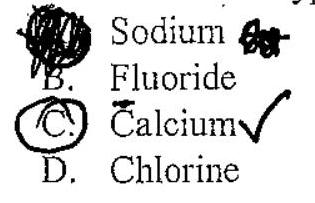
\includegraphics[max width=\textwidth]{2022_11_11_6852287475e47d0e3aceg-04}

$$
\begin{aligned}
&\mathrm{ca}(\mathrm{OCl})_{2} \text { is explosire \& igntuble } \\
&\text { with Activatal Carbon. }
\end{aligned}
$$

\begin{enumerate}
  \setcounter{enumi}{28}
  \item What are the two most important safety concerns when entering a confined space?\\
A. Corrosive chemicals and falls\\
B. Bad odors and claustrophobia\\
C. Extreme air temperatures and slippery surfaces\\
D. Oxygen deficiency and hazardous gases 30. What piece of safety equipment must an operator wear when entering a confined space?\\
A. Boots\\
(B.) Harness\\
C. Gloves\\
D. Croggles

  \item What type of fire extinguisher should be used for fires with live electricity present?\\
A. Class A\\
B. Class B\\
C.) Class C\\
D. Class D

\end{enumerate}

$$
\begin{aligned}
&A \text { - Wareted } \\
&B-\text { Gas } \\
&C \text { - Exiplosine }
\end{aligned}
$$

\begin{enumerate}
  \setcounter{enumi}{31}
  \item Which document provides a profile of hazardous substances?\\
A. CERCLA\\
B. SARA\\
C. CFR\\
D. $\mathrm{MSDS}$
\end{enumerate}

\begin{itemize}
  \item Nuw SDI\\
Materinl\\
$\operatorname{Sin} f=4$\\
Dida shent
\end{itemize}

\begin{enumerate}
  \setcounter{enumi}{32}
  \item What safety measure must an operator follow prior to working on electrical equipment?\\
A. Lock out and tag out all electrical switches\\
B. Put on canvas gloves\\
C. Remove fuses from switch box\\
D. Tell one coworker not to turn on the switch

  \item What is the correct procedure for mixing acid and water?\\
A. Water is added slowly to the acid\\
B. Acid is added slowly to the water\\
Water is added quickly to the acid\\
D. Acid is added quickly to the water

  \item What is the purpose of a pump guard?\\
A. Allows operators to turn off pump in emergency situations\\
B. Notifies operators of excessive temperatures\\
C. Allows operators to pump against a closed discharge valve\\
D. Protects operators from rotating parts

  \item The most important responsibility of an operator is to provide\\
A. Adequate water pressure\\
B. Palatable drinking water\\
C. Adequate amounts of water\\
D. Safe drinking water\\
$-$

  \item To ensure that the water supplied by a public water system meets federal and state requirements, the water system operator must regularly collect samples and\\
A. Test the water at the nearest water testing laboratory\\
B. Determine a sampling schedule based on the lab's recommendations\\
(C.) Send all analysis results to the State periodically\\
D. Count the number of active wells in the system 38. The major source of error when obtaining water quality information is improper\\
A. Sampling\\
B. Preservation\\
C. Tests of samples\\
D. Reporting of data

  \item A composite sample should never be used when sampling for which contaminant?\\
A. Benzene\\
B. Nitrate\\
C. Barium\\
D. Bacteria

  \item When should water guality samples for chlorine residual be analyzed?

\end{enumerate}

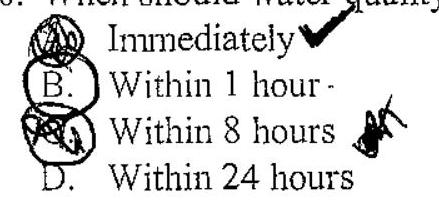
\includegraphics[max width=\textwidth]{2022_11_11_6852287475e47d0e3aceg-06}


\includegraphics[max width=\textwidth]{2022_11_11_6852287475e47d0e3aceg-06(1)}

\begin{enumerate}
  \setcounter{enumi}{40}
  \item How many coliform samples are required per month for a water system serving a population between 25\\
(A.) 1\\
B. 2\\
C. 3\\
D. 4
\end{enumerate}

and 100 ?

\begin{enumerate}
  \setcounter{enumi}{41}
  \item Water laboratory test calculations and results use which system?\\
A English\\
(B.) Metric\\
SWAG\\
D. British

  \item Factors of what number are used in the metric system?\\
A. 5\\
B. 10\\
C. 12\\
D. 64

  \item What is the chemical formula for sulfuric acid?\\
A. $\mathrm{SA}_{2}$\\
B. $\mathrm{H}_{2} \mathrm{SO}_{4}$\\
C. $\mathrm{NaOH}$\\
D. $\mathrm{H}_{2} \mathrm{O}$

  \item Which of the following should not be used to draw a sample into a pipet?\\
A. Mouth\\
B. Bulb\\
C. Pump\\
D. Straw 46. Which of the following are two types of samples?\\
A. Dessicator and gooch\\
B. Wet and dry\\
C. Buret and flask\\
D. Grab and conposite

  \item What two types of devices are used to collect samples?\\
A. Left and right\\
B. Upper and lower\\
C. Automatic and manual\\
D. Gas and diesel

  \item How should samples that cannot be analyzed immediately be maintained until the analysis is conducted?\\
A. Shaken every hour\\
B. Preserved\\
C. Held in an open container\\
D. Stored bottom up

  \item What is the most common method used in labs to test for total coliform and $E$. coli?\\
A. DMA\\
B. Green\\
(C.) Colilert\\
D. Lamp

  \item What test method best determines chemical feed/dosage rates?\\
(A.) Jar\\
B. Turbidity\\
C. Hanmer\\
D. Hardness

  \item An empty atmospheric storage tank is 8 feet in diameter and 32 feet high. How long will it take to fill $90 \%$ of the tank volume if a pump is discharging a constant 24 gallons per minute into the tank?\\
(A.) 7 hours 31 minutes\\
B. 8 hours 21 minutes\\
C. 8 hours 23 minutes\\
D. 9 hours 17 minutes\\

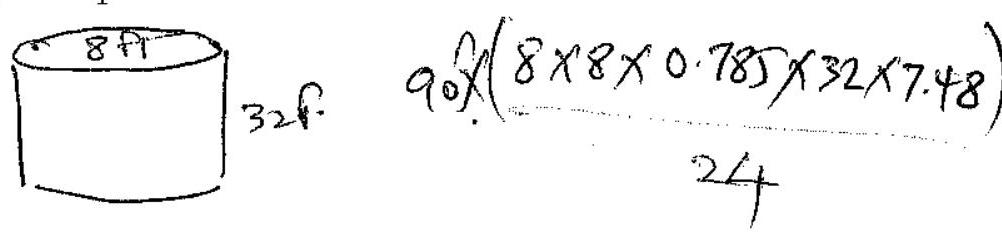
\includegraphics[max width=\textwidth]{2022_11_11_6852287475e47d0e3aceg-07}

  \item Two columns of water are filled completely at sea level to a height of 88 feet. Column A is $0.5$ inches in diameter. Column $B$ is 5 inches in diameter. What will two pressure gauges, one attached to the bottom of each column, read?

\end{enumerate}

$\begin{array}{lrr} & \frac{\text { Column A }}{} & \text { Column B } \\ \text { A. } & 3.8 \mathrm{psi} & 38.0 \mathrm{psi} \\ \text { B. } & 8.8 \mathrm{psi} & 8.0 \mathrm{psi} \\ \text { C. } & 20.3 \mathrm{psi} & 20.3 \mathrm{psi} \\ \text { D. } & 38.0 \mathrm{psi} & 38.0 \mathrm{psi}\end{array}$

\begin{enumerate}
  \setcounter{enumi}{52}
  \item A ditch that is $4.5$ feet wide, 6 feet deep, and 120 feet long has to be dug for a water line. How many cubic yards of material must be removed?\\
(A.) 120 cubic yards\\
B. 240 cubic yards\\
C. 850 cubic yards\\
D. 1,200 cubic yards
\end{enumerate}

$$
\begin{array}{r}
4 \times 6 \times 120=\frac{3240 \text { cuft }}{27} \\
27 \text { curt }=1 \text { wayard }
\end{array}
$$

\begin{enumerate}
  \setcounter{enumi}{53}
  \item How many cubic feet of water will a rectangular tank that is 20 feet long by 15 feet wide and 10 feet high hold?\\
A. 2,000 cubic feet\\
(B.) 3,000 cubic feet\\
C. 4,000 cubic feet\\
D. 5,000 cubic feet

  \item Calculate the chlorine demand using the following data.

\end{enumerate}

\begin{itemize}
  \item Raw water flow is $0.7 \overrightarrow{\mathrm{M} G D}$.
\end{itemize}

-Chlorinator feed rate is $4.0 \mathrm{mg} / \mathrm{L}$.

-Chlorine residual is $1.8 \mathrm{mg} / \mathrm{L}$.\\
A. $0.8 \mathrm{~m} g / \mathrm{L}$\\
(B.) $2.2 \mathrm{mg} / \mathrm{L}$\\
(B. $4.0 \mathrm{mg} / \mathrm{L}$\\
D. $5.8 \mathrm{mg} / \mathrm{L}$

$$
\frac{9 c}{5}+32=32=
$$

\begin{enumerate}
  \setcounter{enumi}{55}
  \item Convert $60.5$ degrees Fahrenheit to degrees Celsius.
\end{enumerate}

$$
4 \cdot-1 \cdot 8
$$

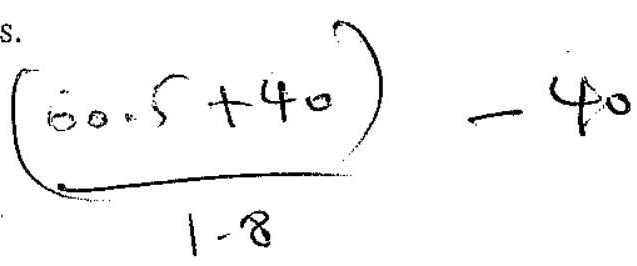
\includegraphics[max width=\textwidth]{2022_11_11_6852287475e47d0e3aceg-08}

\begin{enumerate}
  \setcounter{enumi}{56}
  \item Calculate drawdown, in feet, using the following data.
\end{enumerate}

\begin{itemize}
  \item The water level in a well is 20 feet below the ground surface when the pump is not in operation.
\end{itemize}

-The water level is 35 feet below the ground surface when the pump is in operation.\\
(A.) 15 feet\\
B. 20 feet\\
C. 35 feet\\
D. 55 feet

$$
3 \int-20
$$

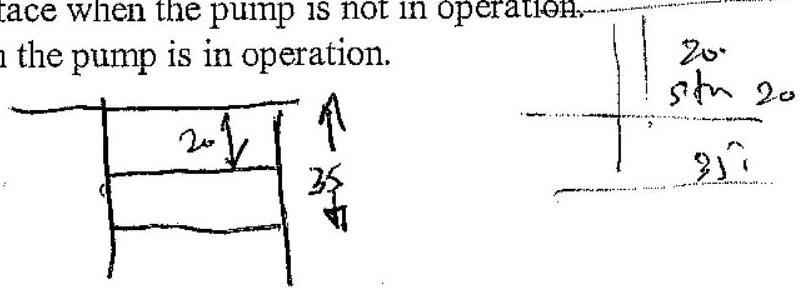
\includegraphics[max width=\textwidth]{2022_11_11_6852287475e47d0e3aceg-08(1)}

\begin{enumerate}
  \setcounter{enumi}{57}
  \item Calculate the volume, in gallons, of a tank that is 75 feet long, 20 feet wide, and 10 feet deep.\\
A. $\quad 15,000$ gallons\\
(B) 112,200 gallons\\
C. 150,000 gallons\\
$75 \times 20 \times 10 \times 7.48$\\
D. 224,400 gallons

  \item How many pounds of a chemical applied at the rate of $3 \mathrm{mg} / \mathrm{L}$ are required to dose 200,000 gallons?\\
A. $3 \mathrm{lbs}$\\
(B.) $5 \mathrm{lbs}$\\
C. $16 \mathrm{lbs}$\\
D. $50 \mathrm{lbs}$

\end{enumerate}

$0.2 \times 8.34 \times 3$ 60. Caiculate the average weekly flow for a system with the following data.

Sunday $-3,000$ gallons Monday - 4,000 gallons Tuesday - 3,500 gallons

Wednesday - 2,000 gallons Thursday - 3,000 gallons Friday - 3,500 gallons

Saturday - 2,000 gallons\\
A. $2,000 \mathrm{gpd}$\\
B. $3,000 \mathrm{gpd}$\\
C. $4,000 \mathrm{gpd}$\\
D. 5,000 gpd

\begin{enumerate}
  \setcounter{enumi}{60}
  \item After a new water main is installed and pressure tested it should be\\
A. Flushed with clean water for 24 hours and put into service\\
(B.) Filled with a solution of 25 ppm to $50 \mathrm{ppm}$ free chlorine for at least 24 hours prior to flushing\\
C. Filled with clean water and allowed to sit for 5 days at full pressure before turning the water into the system\\
D. Photographed so that mapping can be avoided until the system is complete

  \item Chlorine demand is satisfied at the point when\\
(A.) The reaction of chlorine with organic and inorganic materials stops\\
B. Free chlorine residuals reach $2.5 \mathrm{mg} / \mathrm{L}$\\
C. An odor of chlorine is present\\
D. Chlorine reaches the last tap

  \item What chlorine concentration should be produced when disinfecting a well or well pump?\\
A. $25 \mathrm{mg} / \mathrm{L}$\\
(B.) $50 \mathrm{mg} / \mathrm{L}$\\
C. $75 \mathrm{mg} / \mathrm{L}$\\
D. $100 \mathrm{mg} / \mathrm{L}$

  \item When disinfecting a new or repaired main, what is the minimum chlorine residual at the extreme end of the main after:standing for 24 hours?\\
A. $15 \mathrm{mg} / \mathrm{L}$\\
B. $20 \mathrm{mg} / \mathrm{L}$\\
(c.) $25 \mathrm{mg} / \mathrm{L}$\\
D. $30 \mathrm{mg} / \mathrm{L}$

  \item Chlorine will destroy bacteria most rapidly at what $\mathrm{pH}$ ?\\
(A.) $7.5$\\
B. $8.5$\\
C. $9.5$\\
D. $10.5$

  \item What is the process of adding chlorine to water until the chlorine demand has been satisfied called?\\
A. Contact time\\
B. Reliquefaction\\
C. Hypochlorination\\
(D.) Breakpoint chlorination 67. Which of the following pH ranges would deposit a thin film of calcium carbonate on the inside surface of a pipe?\\
A. $2.0-3.0$\\
B. $4.0-5.0$\\
C. $6.0-7.0$\\
(D.) $8.0-9.0$

  \item Where should sodium hypochlorite (liquid bleach) be stored?\\
A. Away from flammable objects, as it is a fire hazard\\
B. Away from equipment that is susceptible to corrosion\\
e. In closed containers at room temperature for no longer than 6 months\\
D. Near the chemical feed pump day tank, to lessen operator handling risks

  \item What is the most important reason for maintaining a continuous positive pressure throughout the distribution system?\\
A. Prevent damage to water meters\\
B. Keep pipe joints sealed\\
(C.) Prevent contamination from backflow\\
D. Maintain chlorine residual

  \item A weir should be used to measure water in which of the following locations?\\
A. Above ground storage tanks\\
B. Household service lines\\
(C.) Open channels\\
D. Water mains

  \item The pumping water level is best defined as the distance from the top of the well to the\\
A. Intake screen of the pump\\
B. Location where the main flow of water enters a well Water after the pump has been operating for a period of time\\
Water level from the start of a pump test to the end of the test

\end{enumerate}

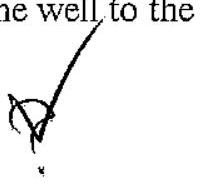
\includegraphics[max width=\textwidth]{2022_11_11_6852287475e47d0e3aceg-10}

\begin{enumerate}
  \setcounter{enumi}{71}
  \item The space between the inner or protective casing and the outer casing or drill hole should be filled with cement grout to a minimum of how many feet?\\
A. 10 feet\\
B. $15 \mathrm{feet}$\\
C. 20 feet\\
D. 35 feet

  \item When bringing community water service to a home with a private well, what is the most positive method of preventing a cross connection between the two systems?\\
A. Residential dual check valve\\
B. Reduced pressure zone backflow preventer\\
C. Complete isolation between the two systems using an air gap\\
D. Pressure vacuum breaker in addition to an $\mathrm{RPZ}$ 74. What is the physical connection, direct or indirect, which provides the opportunity for nonpotable water to enter a conduit, pipe or receptacle containing potable water?\\
A. Well testing\\
B. Pump injection\\
Bell joint clamp\\
(D.) Cross connection

  \item Which of the following causes taste problems and has a rotten egg odor?\\
A. Chlorine\\
B. Benzene\\
C. Nitrate\\
(D.) Hydrogen sulfide

\end{enumerate}

\end{document}